% CAB302 Assignment 2 Report 
% Authors: Alex Butler, Brad Fuller & Joshua O'Riordan
% LaTeX assistance: Vincent Nguyen
% Version 1.2 2019-05-29

% NOTE: May require building twice in order for Contents page to show correctly.

\documentclass[12pt]{article} % This states what size and type of document. Generally leave this as is.

\usepackage{fullpage} % Essential - makes you actually use the whole
\usepackage{amsmath} % Essential - for math
\usepackage{amssymb} % Essential - for math
\usepackage{amstext} % Essential - for math
\usepackage{amsfonts} % Essential - for math
\usepackage{amsthm} % Essential - for math
\usepackage{graphicx} % Essential - for inserting images
\usepackage{hyphenat} % I like this - removes hyphenated continues on new lines
\usepackage{cancel} % I like this - allows use of \cancel{something}
\graphicspath{ {images/} } % I like this - a different way for inserting images
\usepackage{parskip} % I like this - removes first line indentation
\usepackage{microtype} % Added for underfull fixing
\usepackage{float}
% Packages that I use.


\begin{document} % Everything begins and ends with this

\title{Development Report and Documentation
		 \\ \large CAB302 - Assignment 2}

\author {Alex Butler,  Bradley Fuller \& Joshua O'Riordan}
\maketitle

\newpage

\tableofcontents

\newpage

\section{Statement of Completeness}

The solution includes the following features: 
\begin{center}
	\begin{tabular}{|c|c|}
		\hline  \textbf{Drawing - Line} & Complete - Tested Working \\
		\hline  \textbf{Drawing - Plot} & Complete - Tested Working \\
		\hline  \textbf{Drawing - Rectangle} & Complete - Tested Working \\
		\hline  \textbf{Drawing - Ellipse} & Complete - Tested Working \\
		\hline  \textbf{Drawing - Polygon} & Complete - Tested Working \\
		\hline  \textbf{Drawing - Pen Colour} & Complete - Tested Working \\
		\hline  \textbf{Drawing - Fill Colour} & Complete - Tested Working \\
		\hline  \textbf{File Handling - Read} & Complete - Tested Working \\
		\hline  \textbf{File Handling - Write} & Still to be implemented \\
		\hline  \textbf{GUI - Layout} & Complete - Tested Working \\
		\hline  \textbf{GUI - Buttons} & Complete - Tested Working \\
		\hline  \textbf{GUI - Menu Bar} & Complete - Tested Working \\
		\hline  \textbf{GUI - Colour Picker} & Complete - Tested Working \\
		\hline  \textbf{Additional - Undo History} & Complete - Tested Working \\
		\hline  \textbf{Additional - Bitmap Export} & Complete - Tested Working \\
		\hline
	\end{tabular}
\end{center}
By the due date, we were able to complete all of the essential requirements and the required amount of two additional requirements - being Undo History, and Bitmap Export. 

\newpage

\section{Statement of Contribution}

{\large Alex Butler}\\
Alex implemented all of the Shape classes, as well as the Shape interface and enumerator. He also wrote the unit tests for testing each Shape class, and the first iteration of the GUI (mainly for testing purposes). 
\\\\{\large Bradley Fuller}\\
Bradley implemented the file handling and validation classes, as well as the unit testing for said classes. He also wrote and configured the Apache Ant build script, and the TravisCI configuration for continuous integration and delivery to GitHub Releases. He also wrote most of the report, excluding Section 6.
\\\\{\large Joshua O'Riordan}\\
Joshua implemented the final iteration of the GUI, including the general layout, buttons, menu bar and colour picker. He also wrote the additional requirements functionality (being Undo History and Bitmap Export), as well as their respective unit tests.

\newpage

\section{Software Development Practices}

The team utilised Agile's philosophy of iterative and incremental changes, through the use of continuous integration and deployment. This was achieved through the use of TravisCI and GitHub Releases. Whenever a change was made in any branch of the repository, TravisCI would create a temporary Docker container with Ubuntu 16.04 and Oracle JDK 11. All dependencies are then downloaded - in our case, JUnit 5.5.0 and JavaFX, as well as Apache Ant 1.10.6. Ant is used for creating all build folders, compiling the solution, and then running all unit tests (which are stored in the src/tests/ directory). We would then receive a report (via email) of the testing and if any errors occurred. However, if the change was made in the "master" branch of the repository, TravisCI would run Ant's "dist" script, which packages the compiled Java classes in to a JAR file. This JAR file would then be given a version number (which during development was TravisCI's build number) and uploaded to GitHub Releases. Pull requests would also be tested against the "master" branch of the repository to ensure there would be no breaking changes.

Due to other units and other assessment deadlines, we were not able to follow Agile's sprint methodology and strict timing requirements exactly. However, each feature  of the solution was completed in sprints, each being in their own branch in the repository. Once these were complete, the branch would be merged in to master, and work on the next feature could begin. The only exception to this was the File Handling features, as they required the GUI to be fully implemented before they could be merged - however they were tested thoroughly beforehand without the use of a GUI, so the integration was very simple. We also had a kanban board of features that were to be implemented in the project, as well as an automated kanban board for bug triage and fixing.

Test-driven development was also used where possible, especially in the file read and write classes of the solution. The file reading class had over 20 tests of it's own, to make sure that exceptions were being thrown when they should have. Different test cases were used such as invalid commands, invalid co-ordinates, invalid colours, non-VEC file tests, incorrect file types etc.


\newpage

\section{Software Architecture}

As with every Java project, there is a Main class - in this instance, the Main class calls the MainScreen class in order to initialise the GUI. When initialised, the GUI class instantiates the ComponentsClass constructor, which in turn instantiates every Shape class and prepares them for drawing. As well as this, the ShapesEnum enumerator is constructed which includes a list of all shapes. This enumerator is used to aid in drawing shapes for the GUI. The FileRead and FileWrite classes are also instantiated as part of the GUI class - this is in order to read to and write from the Components constructor.

\newpage

\section{Usage of Advanced Object-Oriented Principles}
{\large Abstraction}\\
Some details about abstraction usage.
\\\\{\large Encapsulation}\\
As with most software projects that incorporate the use of object-oriented practice, encapsulation has been used to a large extent in the development of this solution.
\\\\{\large Inheritance}\\
Some details about inheritance usage.
\\\\{\large Polymorphism}\\
Some details about polymorphism usage.

\newpage

\section{Using the Software}

\subsection{Preamble}
This guide is designed to detail and instruct in the usage of the VEC drawing program. Each section describes related functions, such as file handling or keyboard shortcuts.

\subsection{Running the Program}
Upon opening the program a display such as that pictured is shown. 

\begin{figure}[hbtp]
\caption{Blank Display}
\centering
\includegraphics[scale=0.75]{"pictures/window open".PNG}
\end{figure}


The bar on the left hand side is a history bar, and the panel on the right is the location wherein you may draw shapes. Commands are situated in dropdown bars on the top of the program in the menu bar. 

\subsection{Keyboard Shortcuts}
Some commands have keyboard shortcuts, such as Save File. These shortcuts are shown in parentheses after the name of the command. In the case of Save File, pressing ctrl+s (ctrl and s at the same time) will open the dialogue to save the currently displayed picture. Using a keyboard shortcut is the exact same as pressing on the corresponding button.

\subsection{File}
The options under file handle the saving, opening, clearing, and exporting of drawn shapes. The commands available in the dropdown are: New File, Open, Save, and Export BMP.

\subsubsection{New File}
New File clears the program of all history and drawn shapes. This wipes all memory of previous shapes and is irreversible. New File will also disable Undo History if it is already active. The following screenshots demonstrate what pressing New File does.

\begin{figure}[hbtp]
\caption{New Fill - Before Command}
\centering
\includegraphics[scale=0.75]{"pictures/window to be new filed".PNG}
\end{figure}

\begin{figure}[hbtp]
\caption{New Fill - After Command}
\centering
\includegraphics[scale=0.75]{"pictures/window new filled".PNG}
\end{figure}

\subsubsection{Open}
Open allows you to load a VEC file. Loading a VEC file clears the current display of any working progress, and replaces it with that of selected VEC file. Searched file types are filtered by their extension, with the only files shown being those that have the .VEC extension. As Open sets the program to an entirely new image, Undo History is disabled upon the loading of the file.

\begin{figure}[hbtp]
\caption{Open - Example}
\centering
\includegraphics[scale=0.75]{"pictures/openVEC".PNG}
\end{figure}

\subsubsection{Save}
Save is the opposite of Open, in that it allows for the current drawing to be saved to a VEC file. The displayed dialogue allows for the typing of a new file name, however if an existent file is selected that file will be overwritten. Save does not clear the program of previous shapes, allowing you to continuing working without having to open the newly saved file. Like Open, files are filtered so only VEC files are shown. 

Save is disabled if Undo History is active. This ensures that what is saved is always identical to that as is being displayed on the drawing panel.

\begin{figure}[hbtp]
\caption{Save - Example}
\centering
\includegraphics[scale=0.75]{"pictures/saveVEC".PNG}
\end{figure}

\subsubsection{Export BMP}
Export BMP allows for the exporting of what is drawn on the display panel to a bitmap file. Upon pressing the command a window (as shown in Figure 6) is displayed.

\begin{figure}[hbtp]
\caption{BMP - Dimension Options}
\centering
\includegraphics[scale=0.75]{"pictures/bmpFirstWindow".PNG}
\end{figure}

The option on the left (Use drawing board's current dimensions) which is highlighted by default will use the drawing panel's dimensions (in pixels) for the Bitmap. These are the dimensions of the drawing board at the time the Export BMP functionality was called.

The option on the right allows you to enter the width and height in pixels. If the right hand option (Manually enter dimensions) is pressed, a display such as below is shown.


\begin{figure}[H]
\caption{BMP - User Dimensions}
\centering
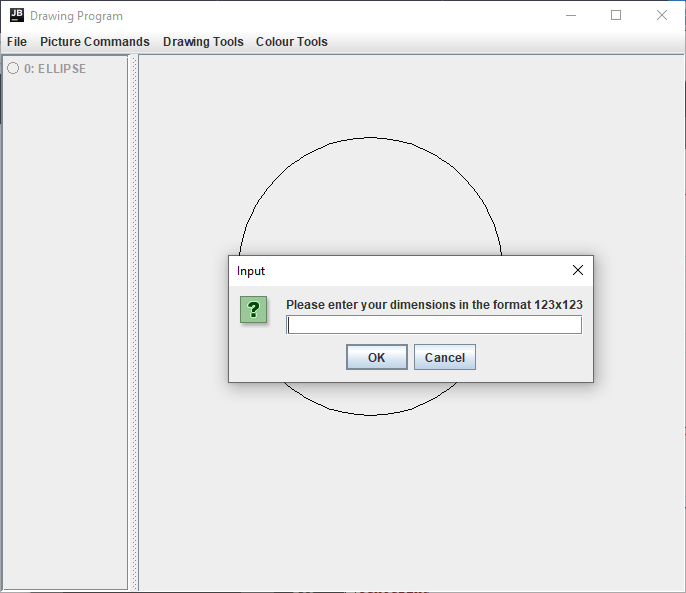
\includegraphics[scale=0.75]{pictures/bmpSecondWindow.PNG}
\end{figure}


The input asks for the dimensions in pixels (simply whole numbers) with width before height. These dimensions must be greater than 0 and less than 6000. Furthermore, the dimensions must be in the pattern of (integers)x(integers). Examples of valid data include 127x127, 1027x720, and 4096x2086. Anything that does not match this (such as 127.7x120 or 12ax129) will result in an error message which will detail the error and return to Figure 7. An example message is shown below.

\begin{figure}[H]
\caption{BMP - User Dimensions Error}
\centering
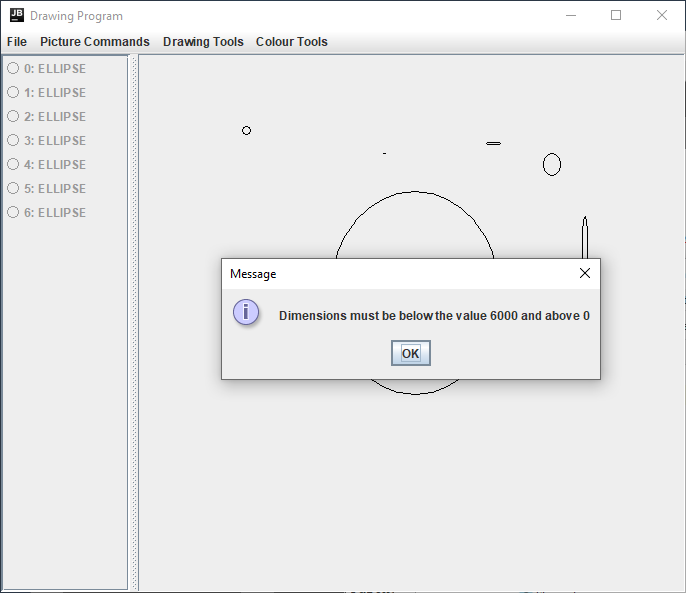
\includegraphics[scale=0.75]{pictures/bmpThirdWindow.PNG}
\end{figure}

If the dimensions are correct, or if the left option (Use drawing board's current dimensions) was selected, then a file saver dialogue will show like below.

\begin{figure}[H]
\caption{BMP - User Dimensions Save File}
\centering
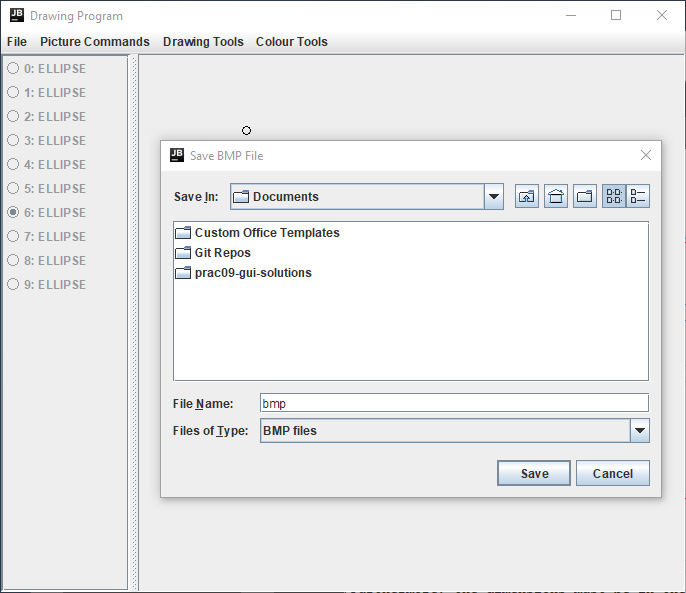
\includegraphics[scale=0.75]{pictures/bmpFourthWindow.PNG}
\end{figure}

Akin to saving VEC files, the dialogue filters for only BMP files. A new file name can be typed, or an existing BMP file can be selected, overwriting it. If you do not add the .bmp extension when typing a new file name, it will be added when the file is written. 

BMP files cannot be displayed by the VEC drawing software, and must be loaded into separate programs (such as Windows 10 Photos) to be displayed.

\subsection{Picture Commands}
Picture Commands handles the navigating of the states of the drawing, or in other words handles how you can view previous iterations of current project. The individual commands are Undo, Show Undo History, and Confirm Selected History.

\subsubsection{Undo}
Undo is analgous to how it operates in programs such as Microsoft Word. Pressing it erases the last shape drawn, both from the drawing panel and the history side bar. An example of this with pictures is below.

\begin{figure}[H]
\caption{Undo - Before Command}
\centering
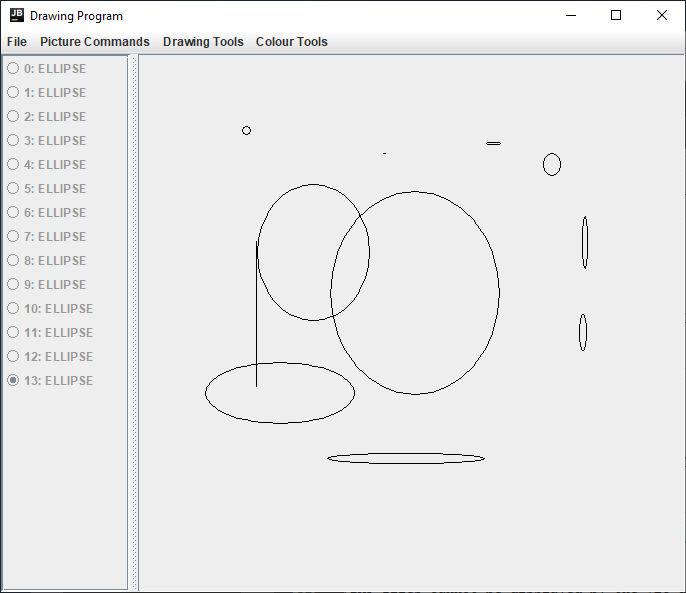
\includegraphics[scale=0.75]{pictures/undoFirstWindow.PNG}
\end{figure}

\begin{figure}[H]
\caption{Undo - After Command}
\centering
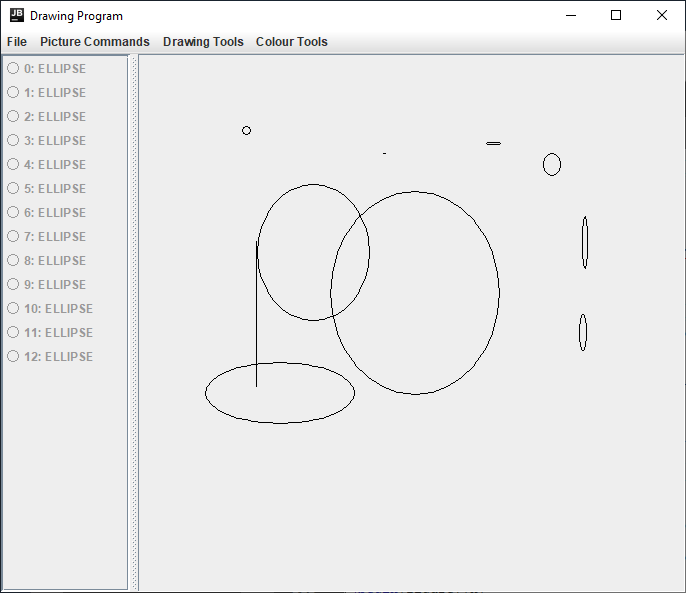
\includegraphics[scale=0.75]{pictures/undoSecondWindow.PNG}
\end{figure}

\subsubsection{Show Undo History}
Show Undo History allows you to see previous states of the picture, analogous to Adobe's Photoshop. Pressing the button will activate this mode, preventing any further drawing on the canvas but allowing you step back to earlier iterations. Clicking on a radio button will show the shape that it corresponds to, as well as every shape prior to it, and none of the shapes after it. To demonstrate:

\begin{figure}[H]
\caption{Show Undo History - Latest State}
\centering
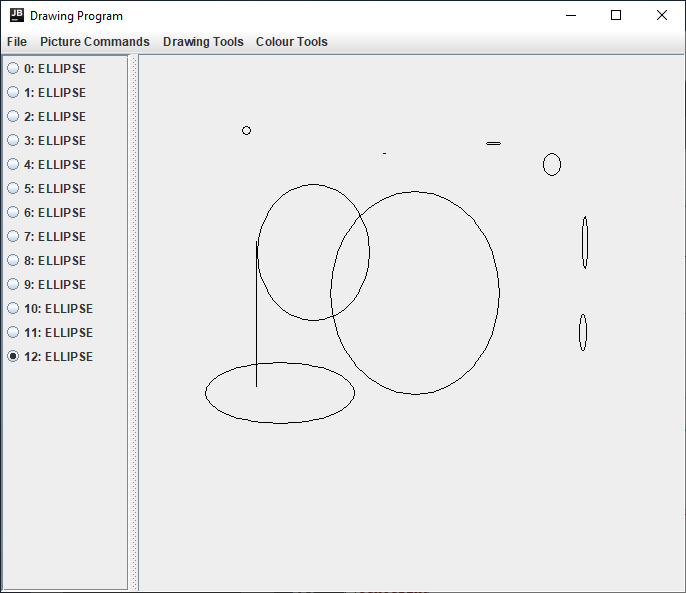
\includegraphics[scale=0.75]{pictures/showUndoFirstWindow.PNG}
\end{figure}

\begin{figure}[H]
\caption{Show Undo History - Middle State}
\centering
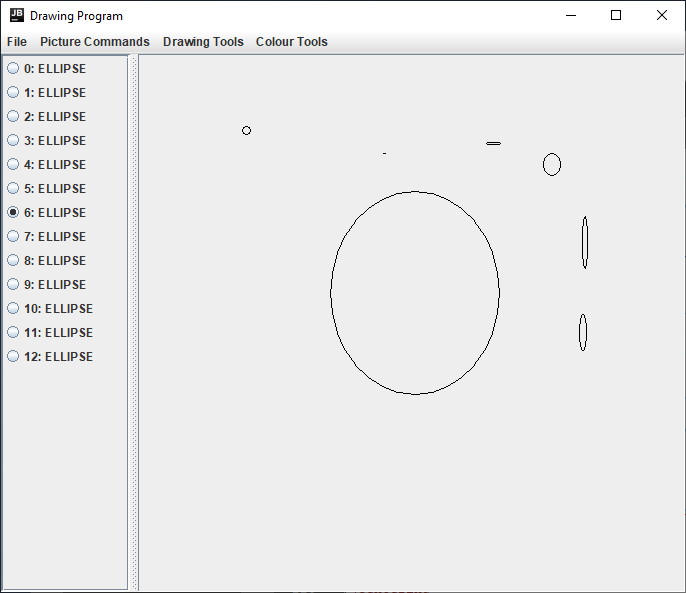
\includegraphics[scale=0.75]{pictures/showUndoSecondWindow.PNG}
\end{figure}

\begin{figure}[H]
\caption{Show Undo History - Earliest State}
\centering
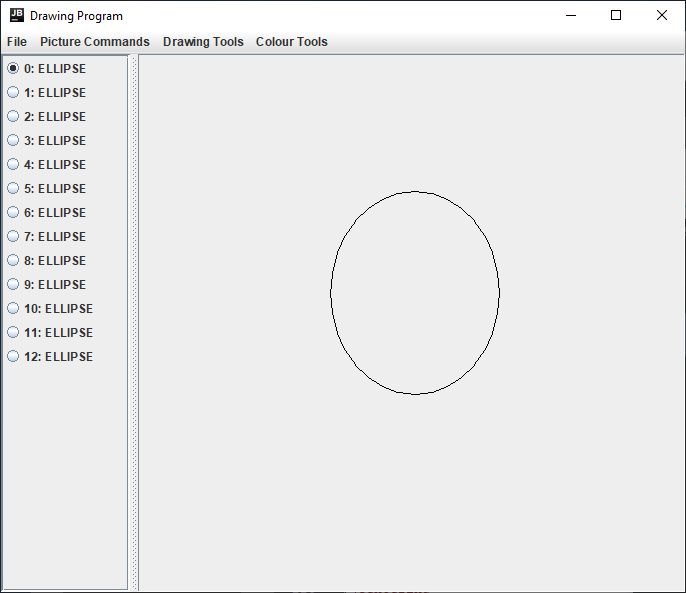
\includegraphics[scale=0.75]{pictures/showUndoThirdWindow.PNG}
\end{figure}

\subsubsection{Confirm Selected History}
Confirm Selected History, if Undo History has been activated by pressing Show Undo History, shows options in regards to saving, disregarding or continuing with the selected state. If Undo History is not active then a warning appears mentioning this and prevents further actions. 

The three options of Confirm Selected History are: Save Selected Picture, Return to Undo History, and Deactivate Undo History. These are shown below.

\begin{figure}[H]
\caption{Confirm Selected History - Options}
\centering
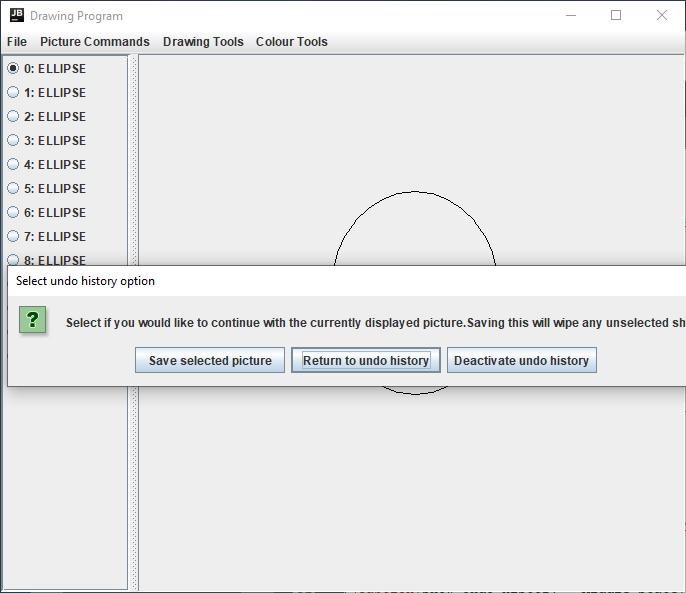
\includegraphics[scale=0.75]{pictures/confirmSecondWindow.PNG}
\end{figure}

Pressing Return to Undo History simply allows you to continue with the Undo History mode.

Pressing Save Selected Picture will re-enable the drawing of new shapes, as well as erasing all states (shapes and associated radio buttons)that are after (or below) the selected shape. This is a permanent action and cannot be undone unless the file was saved with the Save command under File.

Pressing Deactivate Undo History allows for the drawing of more shapes, and sets the drawing canvas to the latest state. 

\subsection{Drawing Tools}
The purpose of this program is drawing, and so these tools are especially important as they allow for a selection of drawing shapes to be chosen. The list of commands is: Plot, Line, Rectangle, Ellipse, Polygon, and Clear Polygon. These commands are divided into sections based upon how they are drawn with the mouse.

\subsubsection{Click, Drag and Release Shapes} 
Line, Rectangle, and Ellipse are all drawn by clicking, dragging and then releasing. After selecting the relevant shape from the dropdown menu, clicking on a point within the drawing canvas will create a new shape of that type (be it line, rectangle or ellipse). Keeping the left mouse button depressed after clicking this spot, dragging the shape will set its orientation, length and if not a line, its size. Releasing the left mouse button will then confirm this shape, and it will be fixed onto the drawing display unless removed with one of the Undo options.

An example of these shapes is below:
\begin{figure}[H]
\caption{Click, Drag and Release Shapes}
\centering
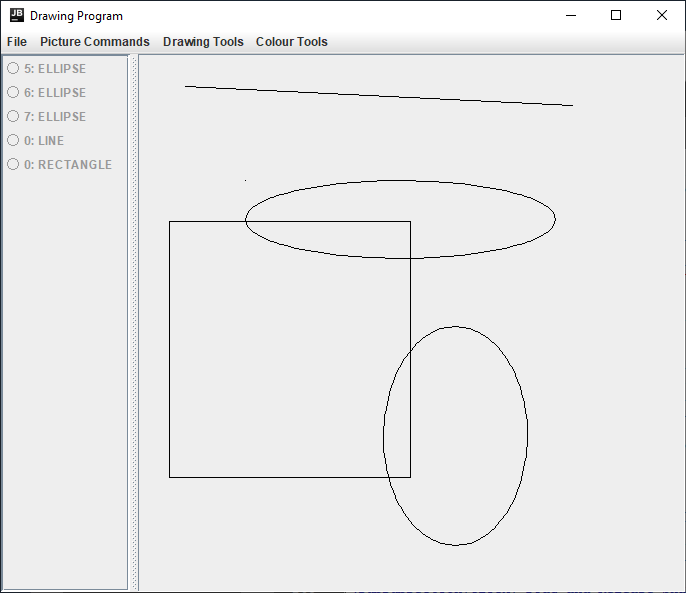
\includegraphics[scale=0.75]{pictures/clickdragreleaseFirstWindow.PNG}
\end{figure}

\subsubsection{Click Shapes}
Plot and Polygon are click shapes. That is, the only mouse interaction used in creating the shape is a click. Plot is a simply dot at the spot of the mouse click.
\begin{figure}[H]
\caption{Click Shapes - Plot}
\centering
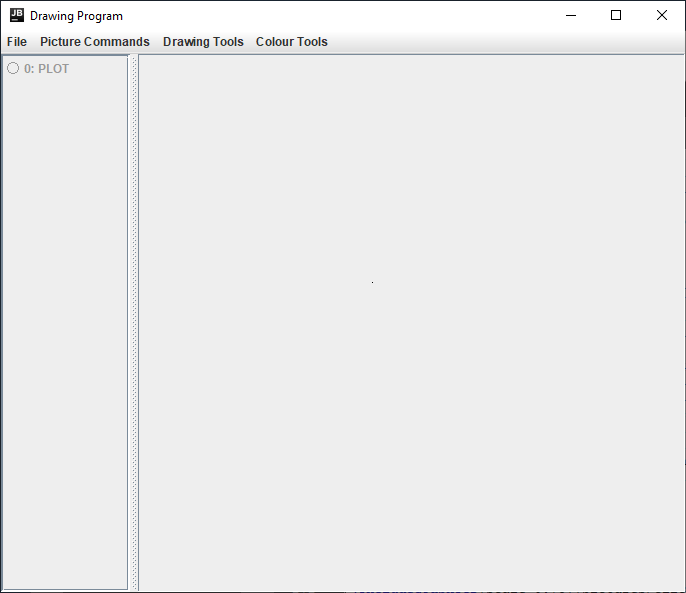
\includegraphics[scale=0.75]{pictures/clickFirstWindow.PNG}
\end{figure}

Polygon is more complex, in that whilst the polygon tool is selected, the latest mouse click will create a point that draws a line to the last point that was clicked (assuming at least two points are clicked). An example of an incomplete polygon is shown:
\begin{figure}[H]
\caption{Click Shapes - Incomplete Polygon}
\centering
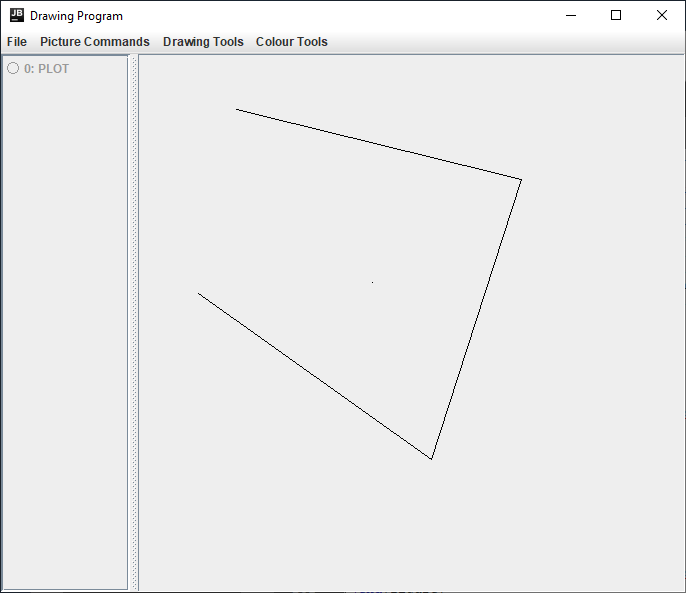
\includegraphics[scale=0.75]{pictures/clickSecondWindow.PNG}
\end{figure}

To complete a polygon you have to connect back to the starting point. In the above example the left-most point of the highest line is the starting point. To complete the polygon, clicking once more on this point is required. The polygon will not be registered in the history side bar until it is completed.
\begin{figure}[H]
\caption{Click Shapes - Complete Polygon}
\centering
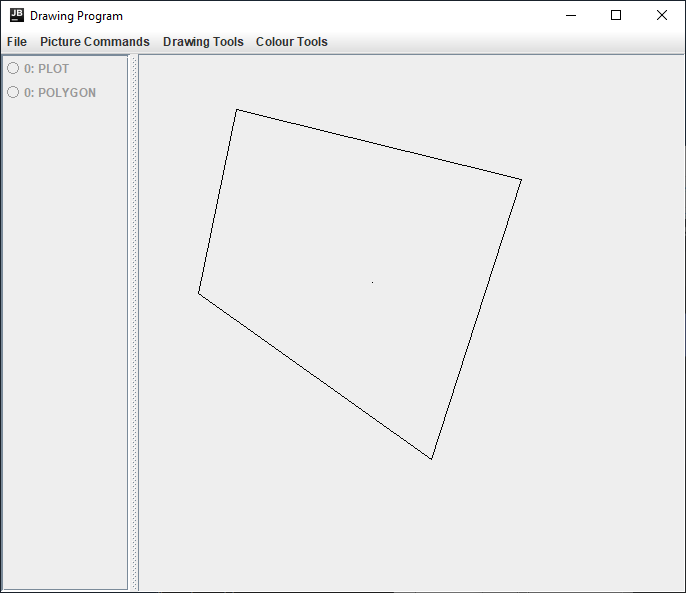
\includegraphics[scale=0.75]{pictures/clickThirdWindow.PNG}
\end{figure}

If one switches to another drawing tool whilst there is an incomplete polygon on the screen, you can draw with the newly selected shape, and then reselect the polygon tool to finish the polygon.

\subsubsection{Clear Polygon}
An incomplete polygon is not registered as a shape, and so as such cannot be removed with the Undo command, saved or affected by Undo History. To remove an incomplete polygon, press Clear Polygon. This will permanently wipe the entire polygon.
\begin{figure}[H]
\caption{Clear Polygon - Example}
\centering
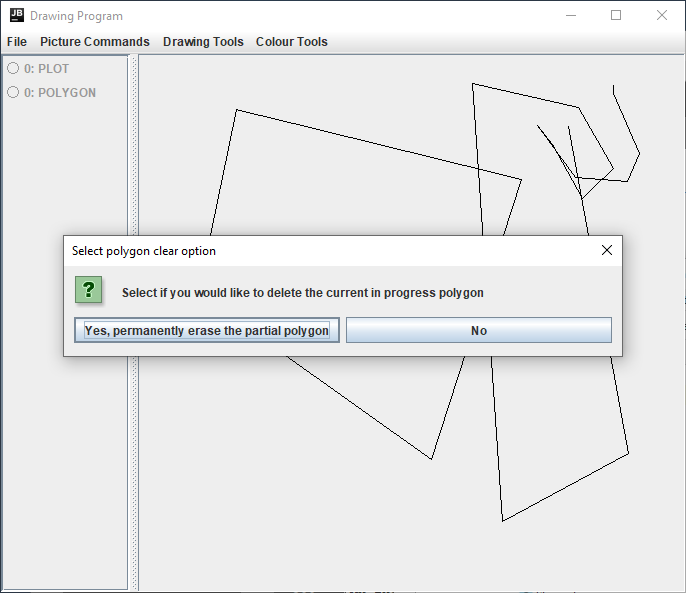
\includegraphics[scale=0.75]{pictures/clickFourthWindow.PNG}
\end{figure}

\subsection{Colour Tools}
Colour Tools allows for changing the colour of both the pen colour (or outline) and the fill colour (which is optional). The options under Colour Tools are Fill Colour, Pen Colour, and Toggle Fill.

\subsubsection{Pen Colour}
Used on every shape, the pen colour sets the colour of the shape's boundary. Upon pressing Pen Colour, a dialogue is shown allowing for one to choose the colour they desire.

\begin{figure}[H]
\caption{Pen Colour - Example}
\centering
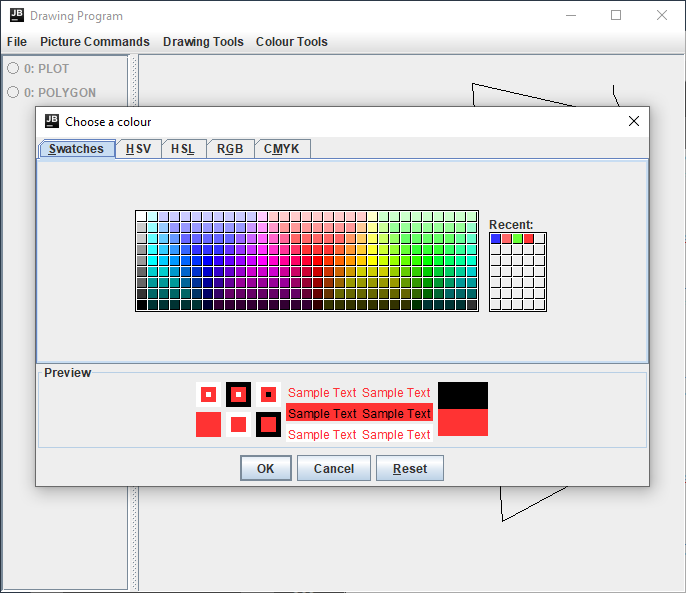
\includegraphics[scale=0.75]{pictures/colourFirstWindow.PNG}
\end{figure}

The currently selected pen colour is shown in the example test. Upon loading the colour chooser this will be the pen colour that is being used for drawing on the canvas, but after selecting a different colour the sample text will change to that colour. Hitting Reset on the dialogue will set the colour back to what it initially was while leaving the dialogue open, whereas Cancel will exit the dialogue whilst keeping the pen colour unchanged. Hitting OK will set the pen colour to the currently selected colour in the chooser.

The recent swatches stores previously clicked on colours (not just those selected), across both the Pen Colour and Fill Colour dialogues. This allows for quick access to colour that are of interest.

Finally, the other tabs (such as HSV) allow for other ways of creating a colour, as opposed to relying on the swatches.


\begin{figure}[H]
\caption{Pen Colour - RGB Example}
\centering
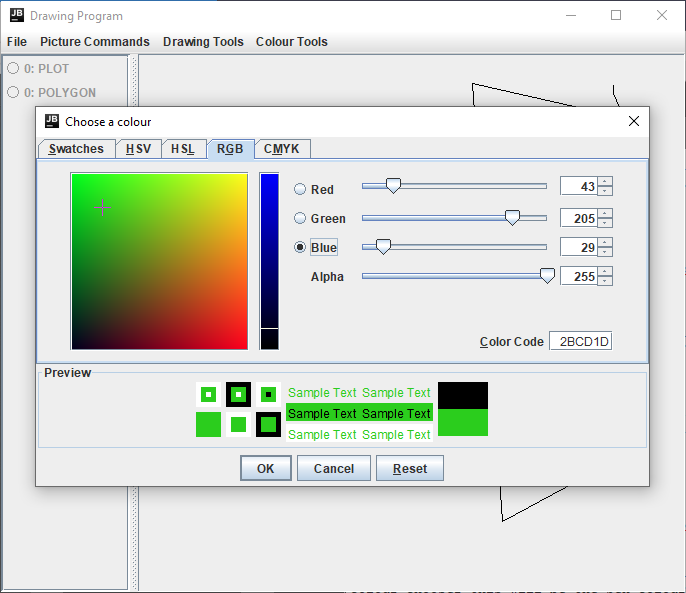
\includegraphics[scale=0.75]{pictures/colourSecondWindow.PNG}
\end{figure}

\subsubsection{Fill Colour}
Fill Colour operates in the same way as Pen Colour. The only difference worth noting is that selecting a fill with OK will not result in the colour being applied as a fill if filling has been disabled with Toggle Fill. 

\subsubsection{Toggle Fill}
This simply toggles whether or not shapes are to be filled when drawn or not. By default they are not, so clicking this for the first time will activate colour filling, and then hitting it again will disable filling, and so forth.

\begin{figure}[H]
\caption{Toggle Fill - No Fill}
\centering
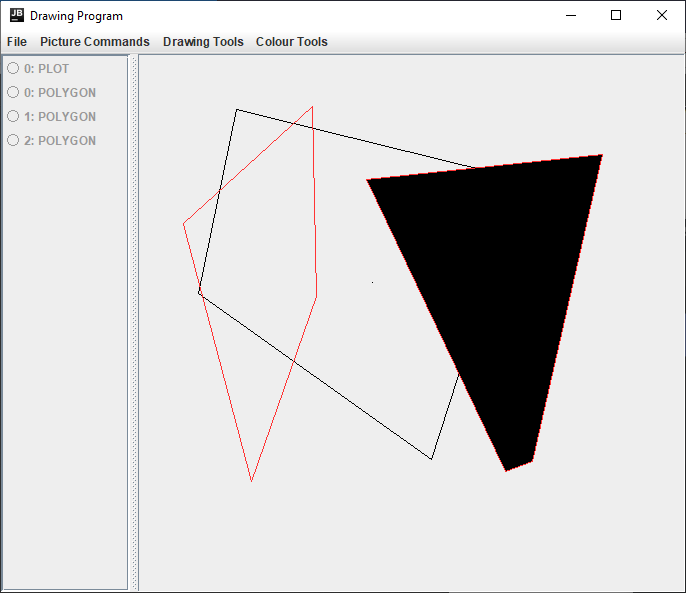
\includegraphics[scale=0.75]{pictures/toggleFirstWindow.PNG}
\end{figure}

\begin{figure}[H]
\caption{Toggle Fill - Fill}
\centering
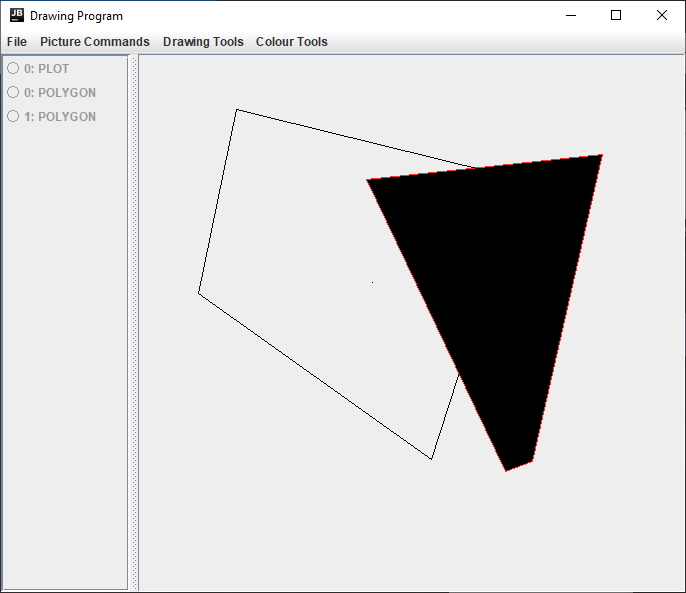
\includegraphics[scale=0.75]{pictures/toggleSecondWindow.PNG}
\end{figure}



\end{document}
